\chapter{Hardware-Anpassungen}

\section{Piplinestufe für Adressports}
Da der Verwendete Prozessor Adress-Isolation ( siehe Kapitel \ref{subsec:add_iso}) einsetzt, sollten die Adressen so lange an einem Port anliegen bis diese geändert werden.
Die für die Schreib- und Lesezugriffe verwendeten Adressen werden jeweils zwischen den Takten an die benötigten Ports angelegt um so zu gewährleisten, dass diese mit der steigenden Taktflanke auch übernommen werden können. Die Auswahl der Ports wird über Enable-Signale geregelt. Werden beispielsweise zwei Instruktionen verwendet die beide an Register-File 1 schreiben, so werden die entsprechenden Adressen an die Ports 0 und 1 angelegt. Sobald diese zu Verfügung stehen, werden diese von den Enable-Signalen freigegeben.\\
Im Fall dieser Architektur tritt nun jedoch Problem auf, denn Adress- und Enable-Signal sind nicht synchron und somit weisen diese ein Zeitversatz, zwischen den beiden Signalen, auf. Dies liegt daran, dass die benötigten Enable-Signale aufwendig berechnet werden müssen und dies eine kurze Verzögerung nach sich zieht. Aus diesem Grund liegt die bereits geänderte Adresse kurze Zeit an dem falschen Adressport an. Sobald das Enable-Signal berechnet wurde, werden die richtigen Adressen angelegt. Dieses Szenario tritt lediglich auf, wenn ein Wechsel in den Enable-Signalen und sich somit die Herkunft der Adressen ändert. Das Beschriebene Problem verursacht eine Erhöhung der Schaltaktivität auf den Adressleitungen und somit auch eine steigende Verlustleistung. %um XXX \%
Um diesem Effekt entgegenzuwirken wurde eine zweite Pipline-Stufe eingebaut. Durch die Verzögerung der Adress- und Enable-Signale ist garantiert, dass die Adressen erst dann an den entsprechenden Ports anliegen, wenn diese benötigt werden. Der zusätzliche Energieverbrauch der Pipeline-Register wird an dieser Stelle nicht weiter untersucht, da der Anstieg der Verlustleistung in den zu vergleichenden Algorithmen identisch ist.

Schaubild Pipelinestufe

Es besteht jedoch eine Möglichkeit, die Pipeline-Stufen zu vermeiden.
Da der Prozessor für ein ASIC entwickelt wird, können die Glitches durch den Einsatz von Buffer behoben werden. Hierzu müssten lediglich die betroffenen Signale mittels eines im ASIC implementierten Buffer verzögert werden. Dieser könnte beispielsweise durch das Einbauen zwei hintereinander geschalteter Inverter realisiert werden. Dabei würde sich die Verzögerung aus der Summe der Gatterlaufzeiten ergeben. Die Anzahl der Inverter-Gatter müsste dann an den Versatz von Adress- und Enable-Signal angepasst werden. 

\section{Neuberechnung der Immediat-Adresse}
Die im Implementierungsteil erläuterten Änderungen sollten keinen Einfluss auf die Daten der auszuführenden Algorithmen haben, jedoch ist beim Vergleich der Implementierungen, eine Abhängigkeit der Daten aufgetaucht.
Diese wurde von Glitches an den Daten-Leitungen verursacht. Diese Veränderung der Daten sind nicht erwünscht und wurden aus diesem Grund mittels Anpassung der Hardware entfernt.
Die Exekution-Stage verwendet für jede Instruktion die dekodierten Adressen aus der Decoding-Stage, hierbei wurde die Source-Adresse für kurze Zeit als Immediat-Adresse interpretiert. Dies führt dazu, dass kurzzeitig Daten aus dem falschen Register gelesen werden. Dies hat zur Folge, dass die falschen Daten an den Register-Ports angelegt werden. Dadurch entstehen Schaltaktivitäten die zu einer höheren dynamischen Verlustleistung an den Daten-Leitungen führen. Um dieses Phänomen zu beheben,  wird eine Neuberechnung der Immediat-Adresse nur dann vorgenommen, wenn auch eine Immediat-Instruktion vorliegt. Hierzu wurde im Decode-Modul des Prozessors verändert. 
Mittels dieser Veränderung, ist die Verlustleistung nun nicht mehr von den Daten abhängig.

\section{Offset-Berechnung für Immediat-Adressen}


\chapter{Evaluation}
\label{chap:evaluation} 
Da die Verlustleistung nicht im Code und zur Laufzeit bestimmt werden kann, musste eine Analyse nach der Ausführung des Codes stattfinden. Die Vorgehensweise ist in Schaubild \ref{fig:flow_power_analyse} abgebildet.

\begin{scriptsize}
	\begin{figure}[htbp] 
		\centering
		\includesvg[width=0.50\textwidth]{evalution_flow}
		\caption{Power Analyse Ablaufdiagramm}
		\label{fig:flow_power_analyse}
	\end{figure}
\end{scriptsize}

Vorerst wird das gewünschte Assembler Programm zusammen mit der Prozessor-Konfiguration in den im Implementierung Kapitel beschriebenen Compiler geladen. Hierbei muss unter Anderem angegeben werden mit welchen Takten der Prozessor taktet und wie gross die Register fuer diesen Fall sind. Außerdem muss dem Compiler die Variante der zu verwendenden Register-Allocation (Tabelle \ref{tab:algo_conifg}) übergeben werden. Nach erfolgreichem compilieren des Codes steht die Binary Datei und der geschedulte Code zu Verfügung. Im Anschluss an diesen Prozess wird die Leistungsanalyse durchgeführt. Hierzu wird die Netzliste des Prozessors und die Binary Datei benötigt. Das Tool \"Prime Time Suite\" von Synopsys analysiert hierbei alle Schaltaktivitäten im Prozessor und gibt anschließend eine detaillierte Übersicht über die Leistungsaufnahme des Prozessors aus. AUSFÜHRLICHER .\\ 
Mithilfe dieses Evalutionsablaufes sind die in diesem Kapitel evaluierten Ergebnisse entstanden.
\section{Testprogramme}
Um den Einfluss der Register-Adressen besser verstehen zu können wurden Assemblerprogramme entwickelt welche den Einfluss von Target-, Source1 und Source2-Register untersuchen.Hierbei sind diese in der Komplexität gestaffelt. In den folgenden Kapiteln wird nun auf die Ergebnisse der einzelnen Programme und deren Erkenntnisse eingegangen.
\subsection{Empirische Tests}
\label{cap:empirischeTests}
Um die aufgestellte Annahme, dass sich die Verlustleistung proportional zur Hamming-Distanz verhält, zu bestätigen, wurden zu Beginn Assemblerprogramme entworfen, die nur mit physikalischen bzw. festen Registern arbeiten.
Ausserdem wurden vorerst der Best- und Worst-Case untersucht, um das maximale Optimierungspotenial zu ermittelen. Das Programm durchläuft dabei alle Möglichkeiten der Allokation, um zum einen die Register-Allokation und die damit verbundene Hamming-Distanz-Berechnung zu testen, zum Andern alle Einflüsse der Register-Adressierung zu ermitteln. Es bestehen für die Target-Register vier und für die Source-Register 16 Möglichkeiten, dabei sind X2-Operationen ausgenommen. Im Worst-Case werden die Register so adressiert, dass die maximale Hamming-Distanz entsteht. Dabei wechseln die Adressen von 0 auf 31 welches der maximalen Hamming-Distanz von fuenf entspricht. Das Programm hat hierbei keinerlei Funktion und besteht aus Gruenden der Übersichtlichkeit aus nur zwei Instruktionen (ADD und OR). Damit keine Einflüsse durch Scheduling oder Daten entstehen, wurden Instruktionen manuell geschedult und den einzelnen Issue-Slots zugewiesen. Somit ist die Anordnung der Assemblerbefehlen für jeden Testfall identisch und der Einfluss ist somit entkoppelt. Im Falle der Datenabhängigkeiten wurden alle Register mit einer Null initialisiert und im Anschluss nicht verändert. Dadurch werden alle Instruktionen mit den selben Daten ausgeführt und somit besteht keine Abhängigkeit der Daten mehr.
Fuer den Fall des Best-Case wurde die Adresse nicht veraendert und immer auf die Adresse 0 gelesen sowie geschrieben.
Das Power-Analyse-Tool zeigt nach dem ausfuehren des Workflows \ref{fig:flow_power_analyse} eine Uebersicht ueber die Leistungsaufnahme des Prozessors an. Hierbei wird die Leistung in Interne-, Schalt- und Leakageleistung aufgeteilt (siehe Abbildung XXX). 

\begin{figure}[htbp] 
	\centering
	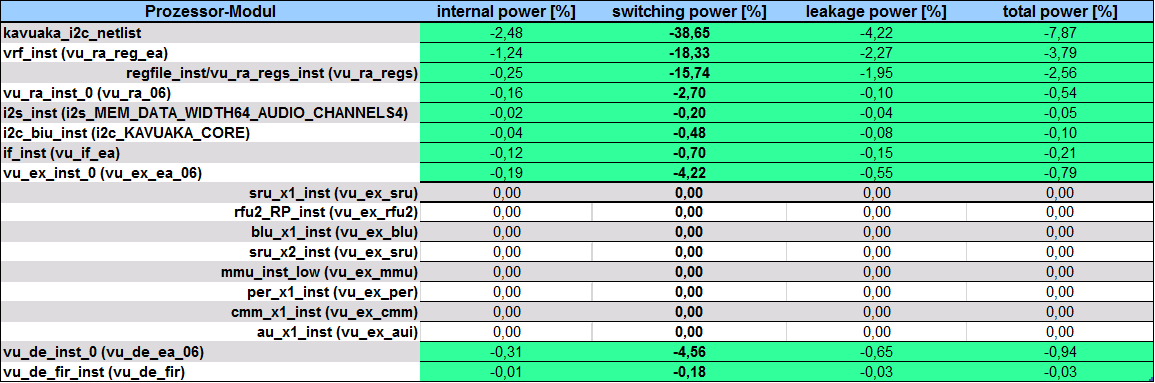
\includegraphics[width=\textwidth]{fig/best_hierarchy.png}
	\caption{Best-Case Leistungseinsparung}
	\label{fig:bes_powersave}
\end{figure}

Um die einzelnen Ergebnisse vergleichen zu können wurden die Programme so entworfen, dass die Hamming-Distanzen für alle Testfälle identisch ausfallen. Ein Beispiel für ein solches Testprogramm, welches den Einfluss der Target-Register testet finden sie im Codebeispiel \ref{code:target_switching_test}.

Start Adressen im Port
Nur eine Variante Adresse 2 auf 0
Varianten aufzaehlen


\begin{algorithm}[H]
	\begin{algorithmic}[1]
		\STATE {:0 \textbf {ADD} V0R2 V0R0 V1R0 \hspace{50pt}:1 \textbf {OR} V0R2 V0R0 V1R0}
		\STATE {:0 \textbf {ADD} V0R0 V0R0 V1R0 \hspace{50pt}:1 \textbf {OR} V1R2 V0R0 V1R0}
		\STATE {:0 \textbf {ADD} V1R0 V0R0 V1R0 \hspace{50pt}:1 \textbf {OR} V0R2 V0R0 V1R0}
		\STATE {:0 \textbf {ADD} V1R2 V0R0 V1R0 \hspace{50pt}:1 \textbf {OR} V1R2 V0R0 V1R0}
		\STATE {:0 \textbf {ADD} V0R0 V0R0 V1R0 \hspace{50pt}:1 \textbf {OR} V0R0 V0R0 V1R0}
		\STATE {:0 \textbf {ADD} V0R2 V0R0 V1R0 \hspace{50pt}:1 \textbf {OR} V1R0 V0R0 V1R0}
		\STATE {:0 \textbf {ADD} V1R2 V0R0 V1R0 \hspace{50pt}:1 \textbf {OR} V0R0 V0R0 V1R0}
		\STATE {:0 \textbf {ADD} V1R0 V0R0 V1R0 \hspace{50pt}:1 \textbf {OR} V1R0 V0R0 V1R0}
		\caption{Codebeispiel Target-Register }
		\label{code:target_switching_test}
	\end{algorithmic}
\end{algorithm}


Um den Einfluss der Adressierung zu ermitteln wurden im Codebeispiel CCC, die Adressen des Target-Registers, von Test zu Test variiert. Um die Source-Register vom Test zu entkoppeln, wurden die Adressen der Register, die nicht untersucht werden sollten nicht verändert. Dadurch entsteht keinerlei Schaltaktivität in den Adressleitungen.

\begin{figure}
	\centering
	\includesvg[width=\textwidth]{switching_power_source1}
	\caption{dynamische Verlustleistung Source 1}
\end{figure}

Um die aufgestellte These zu bestätigen, wurden vorerst zusätzlich nur die Leistung der Adress-Leitungen untersucht. Außerdem wurde der Fokus auf die Untersuchung der Schaltleistung gelegt. Der Test zeigt hierbei, dass bei steigender Hamming-Distanzen die Schaltleistungen der Adress-Leitungen linear zunimmt(siehe Abbildung XXX). Dies bestätigt die Annahme, dass sich die Leistung proportional zur Hamming-Distanz verhält und entspricht somit Formel \ref{eq:dynVerlustleistung} der dynamischen Verlustleistung. Außerdem ist erkennbar, dass keine Schaltleistungen durch Source-Adressen verursacht wurden.
Auffällig ist zudem der Sprung bei einer Hamming-Distanz von 64. Dieser lässt sich dadurch erklären, dass zwar die Hamming-Distanzen identisch sind, aber unterschiedliche Adressleitungen verwendet werden, welche eine größere Lastkapazität aufweisen. Durch die höhere Lastkapazität wird automatisch auch einer größere Leistung benötigt. Dieses Phänomen wird in Kapitel \ref{cap:lastkapa} näher untersucht und erläutert.\\
Abbildung XXX zeigt den Verlauf der Gesamtleistung des Prozessors über der Hamming-Distanz. Auch hier ist eine deutliche Verbesserung erkennbar.

Abbildung Total Power + Switching-power target


Jedoch werden nicht nur Veränderung im Register-File hervorgerufen, denn auch in anderen Modulen ist eine Verbesserung der Verlustleistung zu verzeichnen. Dies liegt daran, dass die Register-Adressen ebenfalls an anderen Modulen Anliegen und dort Veränderungen in der Schaltaktivität verursachen.

Tabelle Hirachy Report

Im Folgenden wurde untersucht, ob diese Abhängigkeiten sich verändern wenn Source- und Target-Register gemeinsam verwendet werden. Hierzu wurden ebenfalls Testfälle generiert, welche die Hamming-Distanzen der Target und Source-Register variiert. Auch hier ist das lineare Verhalten von Hamming-Distanz zu Schaltleistung zu erkennen.


\subsection{Heuristik} 
Da nun die Abhängigkeiten der Register-Adressierung zu der Verlustleistung bewiesen wurde, soll nun verbesserte Heuristik untersucht werden. Hierzu werden wie in Kapitel \ref{cap:empirischeTests} Assemblerprogramme entworfen welche manuell geschedult sind und die Register mit Null initialisiert wurden. Der unterschied zu den empirischen Testprogrammen liegt darin, dass nun ebenfalls virtuelle Register verwendet werden.
Dies hat zur folge, dass die Register-Allokation ein geeignete Zuweisung finden muss und somit die Schaltaktivität der Adresse minimieren kann. Das Testprogramm führt vorerst Addition und Or-Befehle mittels physikalischer Register aus. Hierbei wird dem ersten Issue-Slot die Addition und dem zweiten Issue-Slot eine Or-Operation zugewiesen. Durch das addieren und verodern und anschließende Abspeicherung in physikalische Register, wird eine gewisse Anzahl an Registern fest blockiert und kann nicht für virtuelle Register verwendet werden.(Siehe Abbildung xxx)
Nach dem die Register-Files vorbelegt wurden werden die Instruktionen mit virtuellen Registern begonnen. Ab diesem Punkt ergeben sich Veränderungen in der Register-Allokation. Je nach gewähltem Verfahren, wird nach den physikalischen Registern nach unterschiedlichen Ansätzen gesucht. 

Der Test zeigt hierbei, dass für diesen Testfall die neue Heuristik eine Verbesserung der Hamming-Distanz von XXX\% zu erzielen kann. Diese Verbesserung spiegelt sich ebenfalls in der Schaltleistung wieder.(siehe Abbildung XXX).

SChaubild SChaltleistung heuristik genetischer Algo

\subsection{Genetischer Algorithmus}
Da die Heuristik wie bereits in Kapitel \ref{sec:genetischerAlgorithmus} erwähnt nur die Target-Register auf Schaltaktivität minimiert werden kann, wird nun die Verbesserung der Verlustleistung durch zusätzliches optimieren der Source-Register untersucht. 

\subsection{Datenabhängigkeiten}
Da bis zu diesem Punkt alle Test mit Null vorinitialisierten Registern arbeiten, wird in diesem Kapitel untersucht ob eine Datenabhängigkeit zwischen der Verlustleistung und Daten besteht. Hierzu wurde eine Programm entwickelt, welches zu beginn einige Register mit Daten befüllt. Diese werden im Anschluss mit den selben Instruktionen verarbeitet. Der Unterschied zwischen den Programmen liegt ausschließlich in der Adressierung der Register.  

\section{reelle Testprogramme}
\label{sec:testprogamme}
Um den implementierten Code zu testen und eine reelle Einsparung der Verlustleistungsreduktion zu ermitteln wurden die folgenden Assembler-Programme verwendet. Dabei handelt es sich um Programme die eine häufig Anwendung in Hörgerät-Prozessoren finden. Ausschlaggebend für die Wahl war die Anzahl der verwendeten virtuellen Registern da mit einer hohen Zahl das Verbesserungspotential der Register-Allokation steigt.
\subsection{Beamforming}
Der Beamforming-Algorithmus wird eingesetzt um eine Positionsbestimmung von Schallwellen im Raum durchzuführen und somit eine Ein- bzw Ausblendung von verschiedenen Geräuschen zu gewährleisten und so das Hörerlebnis zu steigern. 

\subsection{emulated floating Point}
Da der verwendete Prozessor keine floating Point Variablen unterstützt, besteht ein Algorithmus der diese emuliert. 




\section{Einfluss der Lastkapazität}
 \label{cap:lastkapa}
Wie bereits in Kapitel \ref{cap:empirischeTests} erwähnt besteht eine Abhängigkeit zwischen Lastkapazität und Verlustleistung. Dies lässt sich auf die Formel der dynamischen Verlustleistung zurückführen \ref{eq:dynVerlustleistung}, laut dieser steigt die Verlustleistung linear mit der Lastkapazität.
Das untenstehende Schaubild \ref{fig:read_port_mux} zeigt wie die Daten aus den Registern an die Read-Ports angelegt werden. Hierbei ist jedes Bit der Register-Adresse für das Schalten eines Multiplexers zuständig. Besteht nun der Fall, dass ein Register mit einer Adresse von 31 ausgelesen werden soll, so müssen alle Multiplexer durchschalten. Dadurch werden die Daten des Registers an den Verwendeten Register-Port weitergeleitet. Wird im Gegensatz hierzu eine niedrige Adresse beispielsweise 0 angefragt, so muss keiner der Multiplexer schalten. Das Signal liegt direkt an dem Read-Port an. Aus diesem Grund benötigen die oberen Adressleitungen mehr Verlustleistung da das Signal eine höhere Lastkapazität aufweist. Dies lässt sich ebenfalls in den Power-Reports nachvollziehen. Dort ist deutlich zu erkennen, dass die oberen Register-Adressen eine höhere Lastkapazität aufweisen. 
\begin{scriptsize}
	\begin{figure}[htbp] 
		\centering
		\includesvg[width=\textwidth]{Read-Port-Mux}
		\caption{Read-Port Multiplexer}
		\label{fig:read_port_mux}
	\end{figure}
\end{scriptsize}

Aus diesem Grund wurde die Fitness Funktion des Genetischen Algorithmus so angepasst, dass die Lastkapazität zusätzlich berücksichtigt wird.

\section{Evaluation}
\label{sec:evalutation_verification}



Parameter sind auf spezielle Algorithmen und koennen nicht pauschalisiert werden.